\documentclass{beamer}

\usepackage[french]{babel}
\usepackage[OT1]{fontenc}
\usepackage[utf8]{inputenc}

\usetheme{Warsaw}

\title{ Introduction au Data Mining}
\author{DNJOMOU YONMBA WILFRIED LOIC CM-UDS-24SCI0999 \\
KENFACK LEONEL CM-UDS-17SCI0998\\
SAGUEU WAKAM DILANE CM-UDS-24SCI1040\\}
\date{Mars 2024}
%\logo{\includegraphics[width=0.2\textwidth]{.\Logo}}

\AtBeginSection[]{
    \begin{frame}
        \tableofcontents[sectionstyle=show/shaded, subsectionstyle=show/shaded, subsubsectionstyle=show/shaded]
    \end{frame}
}

\begin{document}
\frame{\titlepage}
    
    \begin{frame}
        \frametitle{Plan}
        \tableofcontents
    \end{frame}
    
    \section{Définition et Enjeux du Data Mining} 
        \subsection{Définition de la donnee et du Data Mining }
            \subsubsection{Methode de correction de rang un}
        \subsection{motivations }
        \subsection{Objectifs }
        \subsection{Applications réelles }
            
            
            
    
      \begin{frame}
          \frametitle{Définition de la donnee}
          somethings \\
  
        \end{frame}               
    
     \section{Approches et Processus du Data Mining}
        \subsection{Le processus de découverte de connaissances (KDD) }
        \subsection{la méthodologie CRISP-DM }
            
      \begin{frame}
          \frametitle{Le processus de découverte de connaissances (KDD)}
          La découverte de connaissances dans les bases de données (KDD: Knowledge Discovery in Databases), désigne l'extraction non triviale d'informations implicites, jusqu'alors inconnues et potentiellement utiles, à partir de données stockées dans des bases de données.

          \begin{figure}[]
            \centering
            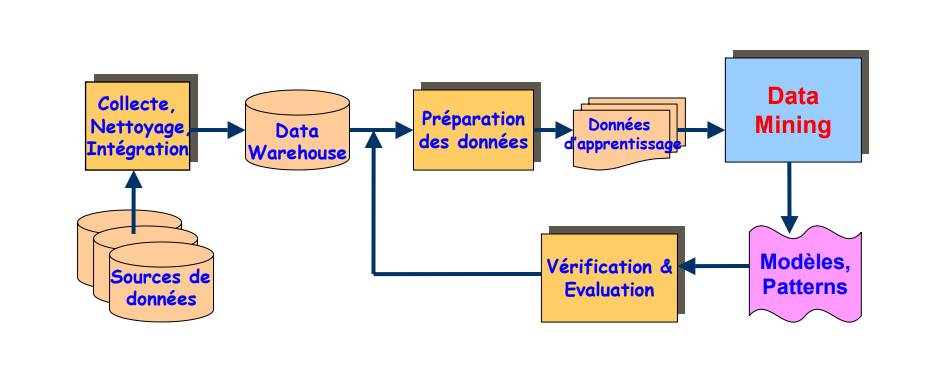
\includegraphics[width=0.75\textwidth]{images/KDD_data_mining.png}
            \caption{Data mining : coeur de KDD.}
            \label{fig:mesh1}
        \end{figure}   
      \end{frame} 
      \begin{frame}
          \frametitle{Le processus de découverte de connaissances (KDD)}
          Le processus de découverte de connaissances dans les bases de données comprend plusieurs étapes, allant de la collecte de données brutes à la production de nouvelles connaissances. Ce processus itératif comprend les étapes suivantes.

          \\
          \begin{enumerate}
            \item \textbf{Nettoyage des données}
            \item \textbf{Intégration des données}
            \item \textbf{Sélection des données} 
            \item \textbf{Transformation des données}
            \item \textbf{Data Mining}
            \item \textbf{Évaluation des modèles}
            \item \textbf{Représentation des connaissances}
           
          \end{enumerate}
           
      \end{frame} 

      \begin{frame}
          \frametitle{la méthodologie CRISP-DM}
          CRISP-DM, qui signifie Cross-Industry Standard Process for Data Mining, est une méthode mise à l'épreuve sur le terrain permettant d'orienter les travaux d'exploration de données.
        \begin{itemize}
            \item En tant que \textbf{méthodologie}, CRISP-DM comprend des descriptions des phases typiques d'un projet et des tâches comprises dans chaque phase, et une explication des relations entre ces tâches.
            \item En tant que \textbf{modèle de processus}, CRISP-DM offre un aperçu du cycle de vie de l'exploration de données.
        \end{itemize}
         
      \end{frame} 

      \begin{frame}
          \frametitle{la méthodologie CRISP-DM}
              \begin{columns}
              \column{0.5\textwidth}
                  \begin{enumerate}
                    \item \textbf{La compréhension du besoin client}
                    \item \textbf{La compréhension des données}
                    \item \textbf{La préparation des données} 
                    \item \textbf{La modélisation ou modeling}
                    \item \textbf{L’évaluation}
                    \item \textbf{ Le déploiement}                   
                  \end{enumerate}
             
                  \column{0.5\textwidth}
                    \centering
                  \begin{figure}[htbp]
                        \centering
                        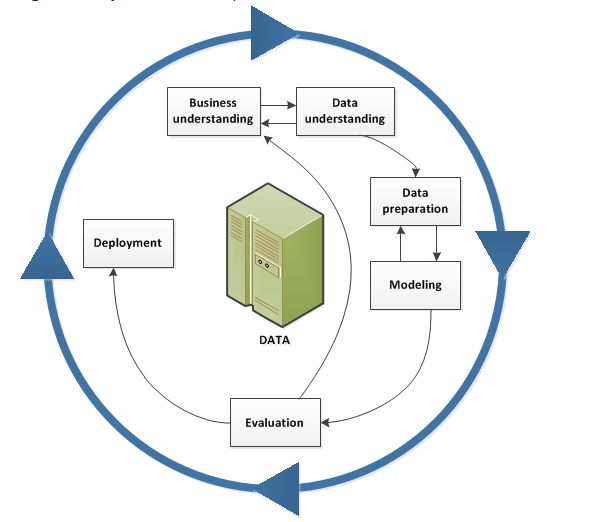
\includegraphics[width=0.75\textwidth]{images/crispdm.png}
                        \caption{Le cycle de vie de l'exploration des données.}
                        \label{fig:mesh1}
                \end{figure}
              \end{columns}
         
      \end{frame} 
      
      
         
     
     
    
        
   
     
      
      
\end{document} 